\section{\textit{Indexing}}
\label{sec:index}

\textit{Indexing} adalah suatu teknik untuk menyusun kata-kata dan mengurangi usaha untuk mencari hal yang berkaitan dengan kata tersebut jika diperlukan, \parencite{database}. Secara umum, indeks banyak digunakan pada buku teks, basis data, dan sistem information retrieval. Seperti salah satu contoh tekniknya adalah \textit{Inverted Index} yang telah dijelaskan pada \ref{sec:invertedindex}.

Terdapat kelebihan penggunaan indeks, diantaranya:
\begin{enumerate}
    \item \textit{Indexing} dapat mempercepat proses pencarian data dengan membuat indeks dan mencocokkan kata kunci dengan indeks tersebut, sehingga mesin dapat menemukan data dengan lebih cepat.
    \item \textit{Indexing} dapat meningkatkan akurasi pencarian dengan menampilkan hasil pencarian yang lebih relevan dengan kata kunci yang dimasukkan.
\end{enumerate}

Namun, ada juga kelemahan dari penggunaan indeks, yaitu sebagai berikut.
\begin{enumerate}
    \item \textit{Indexing} memerlukan ruang penyimpanan tambahan untuk membuat indeks.
    \item Proses pembuatan \textit{indexing} memerlukan waktu, terutama jika data yang akan di-indeks sangat banyak.
\end{enumerate}

Sehingga, dapat disimpulkan penggunaan indeks sangat bermanfaat namun menambahkan biaya.
Pada kasus-kasus dokumen besar, penggunaan indeks pengaruhnya sangat besar karena mesin akan mencari data pada indeks terlebih dahulu sebelum mencari data pada dokumen asli. Hal ini dapat membantu mengurangi waktu pencarian dan menghemat penggunaan memori karena mesin tidak perlu membaca seluruh dokumen untuk menemukan data yang dicari. Namun, apabila \textit{indexing} dilakukan secara berlebihan, akan terdapat banyak indeks yang tidak terpakai dan hanya akan menambah kebutuhan memori.

% Konsep \textit{caching} sendiri adalah menyimpan data yang sering diakses pada level cache atau memori yang lebih dekat dengan CPU agar dapat diakses dengan cepat saat ingin melakukan pencarian, lihat gambar \ref{fig:cache-level}. \textit{Cache} sendiri biasanya memiliki ruang yang terbatas sehingga biasanya membuang data yang sudah tidak diakses sehingga jika dibutuhkan harus dicari ke \textit{storage}. Konsep ini ditiru oleh basis data dan aplikasi \textit{information retrieval} untuk mempercepat proses pencarian dengan memanfaatkan \textit{indexing} untuk mencari (lihat gambar \ref{fig:cache-app}) dan \textit{caching} untuk mengembalikan data yang sering diakses dengan memanfaatkan memori.

% \begin{figure}[h]
%     \centering
%     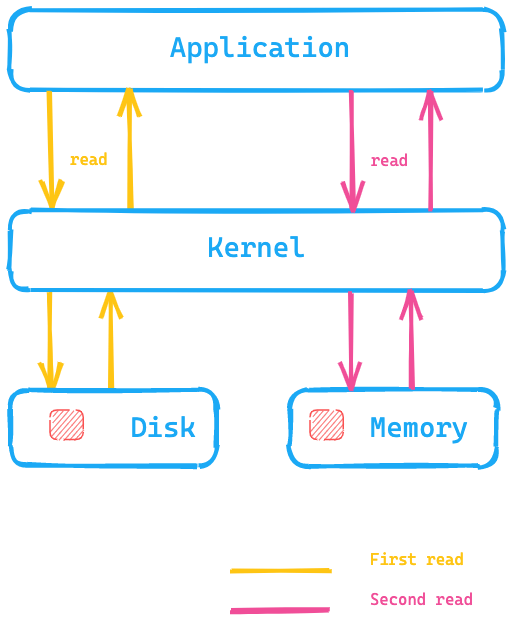
\includegraphics[width=0.5\textwidth]{chapter-2/cache-app.png}
%     \caption{Prinsip Cache pada Aplikasi}
%     \label{fig:cache-app}
% \end{figure}

% \begin{figure}[h]
%     \centering
%     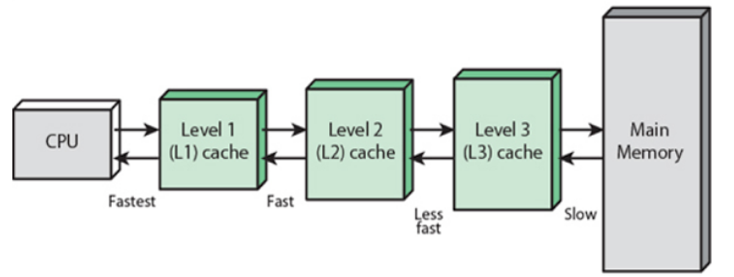
\includegraphics[width=0.5\textwidth]{chapter-2/cache-memory.jpeg}
%     \caption{Level-level pada Cache}
%     \label{fig:cache-level}
% \end{figure}